\setauthor{Martin Hausleitner}
\section{Technologieevaluierung}

Eine grundlegende Komponente des Projektbeginns besteht in der Evaluierung der Technologie. Hierbei wurde bewusst ein angemessener Zeitrahmen zugrunde gelegt, um eine reibungslose und effiziente Entwicklungsphase zu gewährleisten und eventuelle Unzulänglichkeiten im späteren Verlauf des Projekts zu vermeiden. Die definierten Anforderungen umfassen dabei folgende Aspekte:

\begin{itemize}
    \item Entwicklung von Apps für Android und iOS
    \item Möglichkeit zur zukünftigen Veröffentlichung der Anwendung als Webapp
    \item Unterstützung von Datenbankabfragen auf Grundlage von Geo-Koordinaten
    \item Integrierte Authentifizierungs- und Autorisierungsschicht
    \item Realtime-Datenbank, um Echtzeit-Chatrooms für Konversationen zu führen.
\end{itemize}

\subsection{Frontend}

Im Bereich der Frontend-App-Entwicklung stehen verschiedene Möglichkeiten zur Verfügung, um eine App zu programmieren:
\begin{itemize}
    \item Native Entwicklung für jede Plattform (iOS, Android, Web)
    \item Nutzung eines Frameworks für plattformübergreifende Entwicklung von Apps
\end{itemize}

Die native Entwicklung für verschiedene Plattformen wie iOS, Android und Web ermöglicht die spezifische Programmierung einer App in der nativen Sprache der Plattform. Dabei werden für iOS-Apps die Programmiersprache Swift und für Android-Apps Java oder Kotlin verwendet, während für Web-Apps HTML, CSS und JavaScript zum Einsatz kommen.

Durch die native Entwicklung kann eine optimale Performance der App erreicht werden, da sie die native Funktionalität des Geräts vollständig nutzen kann. Entwickler haben die Möglichkeit, auf alle nativen APIs zuzugreifen und die Benutzeroberfläche der App an das jeweilige Betriebssystem anzupassen. Dadurch kann eine höhere Benutzerfreundlichkeit und eine bessere Integration in das Betriebssystem erreicht werden.

Allerdings erfordert die native Entwicklung spezialisierte Kenntnisse in den verschiedenen Plattformen und Programmiersprachen. Mehrere Entwickler mit unterschiedlichen Fachkenntnissen sind möglicherweise erforderlich, um die App für verschiedene Plattformen zu entwickeln. Dadurch kann die native Entwicklung teurer und zeitaufwändiger sein als andere Entwicklungsansätze.

Ein Framework für plattformübergreifende Entwicklung ermöglicht die Erstellung einer einzigen Codebasis, die auf verschiedenen Plattformen wie iOS, Android und dem Web ausgeführt werden kann. Ein solches Framework nutzt häufig eine gemeinsame Programmiersprache wie JavaScript und bietet eine Vielzahl von Bibliotheken und Tools, um die Entwicklung zu erleichtern. Das Framework ermöglicht es Entwicklern, schnell und effizient Apps zu erstellen, ohne sich mit den Unterschieden in den Plattformen und Programmiersprachen auseinandersetzen zu müssen. Ein weiterer Vorteil von Frameworks für plattformübergreifende Entwicklung besteht darin, dass sie eine schnellere Markteinführung ermöglichen und den Entwicklungsaufwand reduzieren können. Allerdings kann die Verwendung eines Frameworks die Performance beeinträchtigen, da es schwierig sein kann, die App für jede Plattform zu optimieren.

Als Resultat einer schnellen Entscheidung wurde festgelegt, dass die Bewältigung dieser Aufgabe nicht durch native Programmierung erfolgen soll. Die mangelnde Vertrautheit aller Teammitglieder mit den Plattformen würde zu einem doppelten Arbeitsaufwand führen, der für ein kleines Team von lediglich drei Personen unverhältnismäßig wäre.

\begin{figure}[htbp]
    \centering
    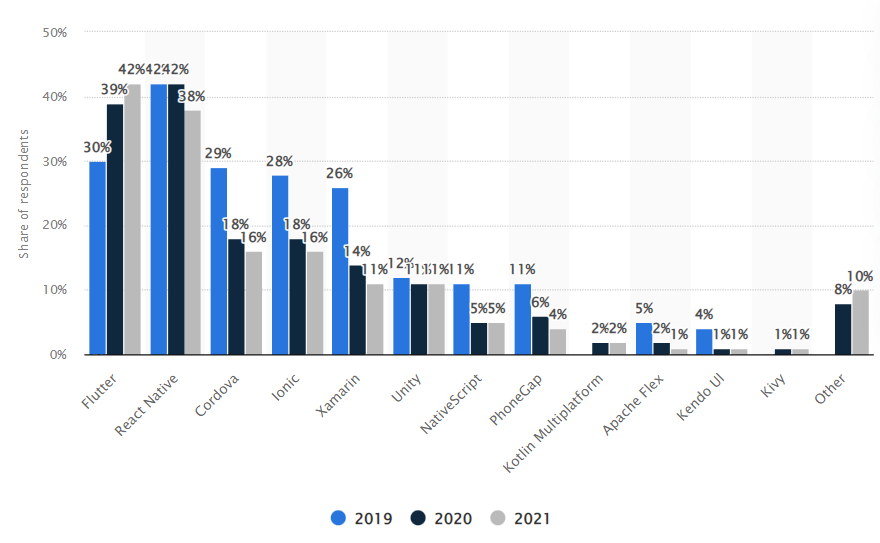
\includegraphics[width=1\textwidth]{pics/cross-platform-statisitics.png}
    \caption{Statistiken zur plattformübergreifenden Nutzung von Statista \cite{statista-software-developer-working-hours} }
    \label{fig:cross-platform-stats}
    % \source{Quelle: Statista (https://www.statista.com/statistics/869224/worldwide-software-developer-working-hours/)}
\end{figure}

Um eine effiziente und plattformübergreifende Entwicklung sicherzustellen, fiel die Wahl auf die Verwendung eines Cross-Platform-Frameworks. Dabei wurde die Statistik in Abbildung \ref{fig:cross-platform-stats} herangezogen, um die am häufigsten genutzten Plattformen zu ermitteln. Es stellte sich heraus, dass Flutter mit 42 Prozent das am meisten verwendete Framework ist und die Tendenz steigend ist. React Native belegt mit nahezu gleicher Beliebtheit den zweiten Platz.

\begin{figure}[h]
    \centering
    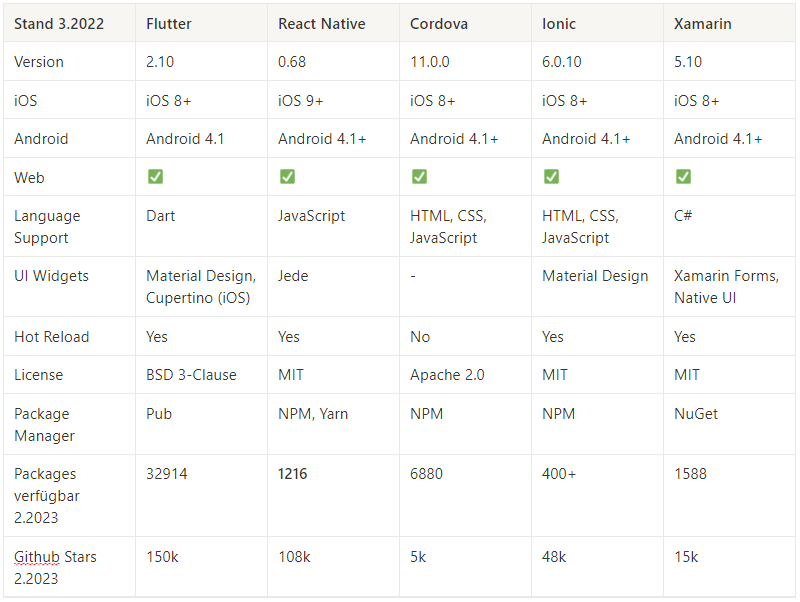
\includegraphics[width=1\textwidth]{pics/framework-comp.png}
    \caption{Vergleich der mobilen Frameworks nach Stand 3.2022 \cite{flutter, react-native, cordova, ionic, xamarin}}
    \label{fig:framework-comp}
\end{figure}

Im Rahmen der vorliegenden Untersuchung wurden die wichtigsten Informationen zu verschiedenen Frameworks in einer Vergleichstabelle zusammengefasst. Es wurde dabei festgestellt, dass sämtliche Plattformen in der Lage sind, die gestellten Anforderungen zu erfüllen.

Insbesondere hat das Framework Xamarin aufgrund der jahrelangen Programmiererfahrung des Teams mit der Sprache C\# ein gewisses Interesse geweckt. Es ist jedoch zu erwähnen, dass auch das Framework Dart aufgrund der ähnlichen Syntax zu C\# eine geeignete Option für das Team darstellt.

\paragraph{Programmiersprachen}\mbox{} \\
React Native ist zwar in JavaScript geschrieben, aber man kann keine React-Komponenten importieren und verwenden. Wenn man jedoch bereits Erfahrung mit React.js hat, kann man sich als Entwickler leichter in React Native einarbeiten. Die letzten beiden Plattformen Cordova und Ionic basieren auf HTML, CSS und JavaScript, was den Vorteil bietet, dass man auf jede JavaScript-Library zugreifen kann.


\paragraph{UI Widgets}\mbox{} \\
Flutter hat als UI-Widget-Library sowohl Material Design 2 und 3 als auch eine iOS Library, die das native iOS-Design 1:1 abbildet. Dadurch kann der Nutzer den Unterschied zwischen nativen und Flutter-Designs kaum erkennen. Xamarin hat ebenfalls eine UI-Library namens Xamarin.Forms, die auf allen Plattformen funktioniert und native UI-Libraries für jede Plattform enthält.

\paragraph{Hot Reload}\mbox{} \\
Ein wichtiger Faktor bei der Wahl des Frameworks ist auch der Hot Reload. Cordova bietet diese Funktion nicht, alle anderen Plattformen hingegen schon, was für uns ein dealbreaker ist.

\paragraph{Package Manager}\mbox{} \\
In der vorliegenden Vergleich wurden verschiedene Package-Manager miteinander verglichen. Nach sorgfältiger Analyse hat sich gezeigt, dass der Package-Manager von Flutter am überzeugendsten ist. Ein ausschlaggebender Faktor hierfür war, dass jeder einzelne Package eine Beispielanwendung beinhaltet. Zudem bietet der Package-Manager die Möglichkeit, durch die Verwendung von Pub Points die Leistung und Qualität des Packages anhand verschiedener Kriterien zu bewerten. Ein weiterer Vorteil besteht darin, dass man leicht erkennen kann, welche Plattformen das jeweilige Package unterstützt. Zusammenfassend lässt sich sagen, dass der Package-Manager von Flutter aufgrund seiner umfangreichen Funktionen und Tools eine herausragende Wahl darstellt.


Obwohl npm der meistgenutzte Package-Manager ist, ist er nicht spezifisch auf ein bestimmtes Framework ausgerichtet und es fehlen einige Funktionen, die Pub hat. In der C\#-Entwicklung ist NuGet bereits bekannt, jedoch wirkt er veraltet und weist ebenfalls einige Funktionslücken im Vergleich zu Pub auf.

\paragraph{Packages}\mbox{} \\
Ein weiterer wichtiger Faktor bei der Wahl des Frameworks sind die verfügbaren Packages. Flutter bietet hier eine große Auswahl, wobei zu beachten ist, dass bei Frameworks, die auf JavaScript basieren, auf alle JavaScript-Libraries zugegriffen werden kann. Insgesamt sind die meisten Flutter-Packages auf mobile Apps ausgerichtet.

\paragraph{Github Stars}\mbox{} \\
Die Community wurde anhand der Anzahl der Github-Stars gemessen, wobei Flutter mit gut einem Drittel vor React Native liegt. Obwohl Flutter noch nicht so lange auf dem Markt ist, spricht dies dafür, dass Entwickler mit Flutter sehr zufrieden sind.

\subsubsection{Performance}\mbox{} \\
Die Performance ist ein wichtiger Faktor bei der Nutzung von Cross-Platform-Frameworks, da sie aufgrund ihrer Nicht-Nativität variieren kann. In einem Forschungspapier \cite{Anwar2021} wurden alle genannten Plattformen bis auf Cordova verglichen, wobei ein aussagekräftiger Vergleich in Punkt 2.6 durchgeführt wurde. Die Ergebnisse zeigen, dass Flutter in Bezug auf die Performance den ersten Platz belegt, gefolgt von React Native auf Platz 2. Im Gegensatz dazu schneidet Xamarin in diesem Vergleich nicht so gut ab. Die letzte Position nimmt Iconic ein, was aufgrund der Tatsache, dass es lediglich eine HTML-, CSS- und JavaScript-Seite in einem Webview anzeigt, nachvollziehbar ist. Im Vergleich zu den anderen Plattformen kann es aufgrund des Fehlens eigener Renderer nicht mithalten.
Wichtig ist zu beachten, dass die Performance-Tests im Dezember 2021 durchgeführt wurden und seitdem hat sich die Geschwindigkeit des Frameworks bis zum aktuellen Zeitpunkt erheblich verbessert.


\subsection
{Backend}
Durch Martin Hausleitners umfassende Kenntnisse in verschiedenen Backend-Technologien wurde die Entscheidungsfindung für das Projekt erleichtert. Bei der Auswahl lag der Fokus auf 'Backend-as-a-Service'-Plattformen, da diese bereits viele Funktionen implementiert haben und das Team dadurch nicht alles von Grund auf programmieren musste.

Bei der Auswahl für das Projekt wurden drei Technologien berücksichtigt: Supabase, Firebase und Appwrite. Jede dieser Optionen stellt SDKs für Flutter und React Native bereit. Zudem verfügen alle über eine Datenbank, die Geoqueries unterstützt, die für das zentrale Merkmal des Radius der Beiträge benötigt wird. Zusätzlich bietet jede Plattform eine Speicherlösung für Beitragsfotos und andere Funktionen.

Supabase hat zum Zeitpunkt der Evaluierung im Februar 2022 jedoch noch keine Cloud-Functions wie Firebase und Appwrite, was es schwierig machte, eine robuste Business-Logik umzusetzen. Obwohl Supabase am 1. April 2022 experimentell Edge Functions eingeführt hat, ist dies für eine Produktions-App nicht empfehlenswert.

Somit verblieben Appwrite und Firebase als die beiden vielversprechendsten Optionen. Obwohl Appwrite in Bezug auf die Funktionen nicht mit Firebase mithalten konnte, spricht für Appwrite, dass es zu 100 Prozent Open Source ist, während Firebase Closed Source ist. Da noch keine endgültige Entscheidung bezüglich des Cross-Platform-Frameworks getroffen wurde, fiel es nun leichter, sich für Firebase zu entscheiden, da es das beste Flutter-SDK aufwies, was an den verfügbaren Features erkennbar war.

\section{Technologieentscheidung}
Die Kombination von Flutter und Firebase harmonieren gut. Flutter ist schnell und hat eine breite Palette von Erweiterungen für mobile Anwendungen sowie eine starke Community. Flutter wird voraussichtlich Marktführer, was ein gutes Gefühl bezüglich der Entscheidung gibt. Zu Beginn gab es Zweifel bei der Arbeit mit Flutter aufgrund der vielen Klammern, die schnell unübersichtlich wurden. Jedoch konnte die Herausforderung dank der super VS Code-Integration mit einem Reformat-Feature gemeistert werden. Auch nach einem Jahr Entwicklung mit Flutter ist es immer noch beeindruckend, wie einfach Features zu implementieren sind und wie straight-forward die Entwicklung ist. Der Syntax von Dart, der Programmiersprache hinter Flutter, ist schnell erlernbar und ermöglicht es, schnell viele Programmierpatterns zu beherrschen.

Firebase hat sich als effektive Wahl erwiesen aufgrund der schnellen und einfachen Entwicklungsmöglichkeiten. Die Skalierung wird automatisch gehandhabt, was ein großer Vorteil ist. Firebase bietet nach wie vor viele erstklassige Features. Allerdings gibt es zwei Nachteile, die die Entscheidung für das Backend beeinflussen könnten. Die Firestore-Datenbank hat keine integrierte Suchfunktion, weshalb Algolia verwendet wurde. Algolia bietet fortgeschrittene Suchfunktionen, die andere Datenbank-Suchmaschinen nicht haben, aber es ist keine perfekte Lösung. Transparenz und Open Source sind wichtige Themen in der Diplomarbeit. Firebase ist allerdings Closed Source, was die bei der Transparenz einschränkt. Aus diesem Grund würde aktuell Supabase bevorzugt, da es Cloud Functions und eine Open-Source-Option bietet. Supabase verwendet PostgreSQL, das bereits eine Suchfunktion integriert hat.
